%!TEX root = ../scivis_lbaakman_bvanloon.tex
In this section the main methods for colormapping are discussed. In \cref{sub:texture_mapping} we discuss \emph{texture mapping}, the method used to map scalar values to colors. Next \cref{ss:colormaps:parameterization} considers the parametrization of colormaps and explains how the number of colors and the saturation can influence the quality of a colormap. Last \cref{ss:colormaps:applying} shows how colormaps are applied to scalar data.

\subsection{Texture Mapping} % (fold)
\label{sub:texture_mapping}
To implement the colormaps \emph{texture mapping} is used. The general pipeline of texture mapping is as follows.
\begin{enumerate}
	\item First the scalar values are sampled for each vertex in the simulation grid.
	\item Next the vertices of the triangulation of the simulation grid is passed to the vertex shader with the associated scalar values.
	\item The vertex shader normalizes scalar values associated with the vertices using a given range of the scalar values creating texture-coordinates for every vertex.
	\item The texture-coordinates are passed to the fragment shader and automatically interpolated by OpenGL.
	\item Next each fragment is rendered by the fragment shader, using the (interpolated) texture-coordinates to lookup the right texture (color) in the colormap.
\end{enumerate}
The end result is a piecewise-linear reconstruction of the (sampled) simulation values. By interpolating the texture coordinates, interpolation of colors is prevented.  This means that no false colors are displayed in the visualization. This is also the main motivation for the choice of texture mapping. The alternative (naive) method of vertex-based colormapping can result in colors that do not correspond with the actual scalar values or even worse, colors that are not in the colormap. These problems are prevented by using texture-based colormapping resulting in a true representation of the scalar values for every pixel.

By using texture mapping a colormap can be generated by constructing a 1D texture that represents the range of colors that are associated with the normalized scalar values. By using the normalized scalar value as index of this 1D texture the corresponding color can be retrieved. By using this approach a colormap can be added to the visualization by providing its 1D texture.

\subsection{Parameterization of Color Maps}
\label{ss:colormaps:parameterization}
Given a colormap scheme there are two parameters which can influence the final map. The number of colors and the saturation of the colors.

\subsubsection{Number of Colors} % (fold)
\label{ssub:number_of_colors}
The number of colormap influences how smooth the colormap looks. When the number of colors in a colormap is low, there is a relatively large difference between the scalar values associated with two neighboring colors in the colormap. This large step will be present in the visualization causing sharp edges between areas with different scalar values. An example of this so called banding effect is given in figure \ref{fig:colormaps:banding} which shows the difference between two colormaps that uses the same color-scheme with one containing 20 colors and the second containing 256 colors. Here we can see that \cref{fig:colormapping:banding:20} shows distinct bands of colors, while \cref{fig:colormapping:banding:256} has smooth transactions between the colors. In our application the user can select the desired number of colors between the range $2 - 256$, making it possible to change the number of colors depending on the desired output. The default value is set to 256 colors, in general the scalar values have continues transitions meaning we need a smooth colormap to avoid color-banding, as that would suggest sharp transitions and a discreteness of the data that is not present.
\begin{figure}[tb]
	\centering
	\begin{subfigure}[t]{0.4\textwidth}
		\centering
		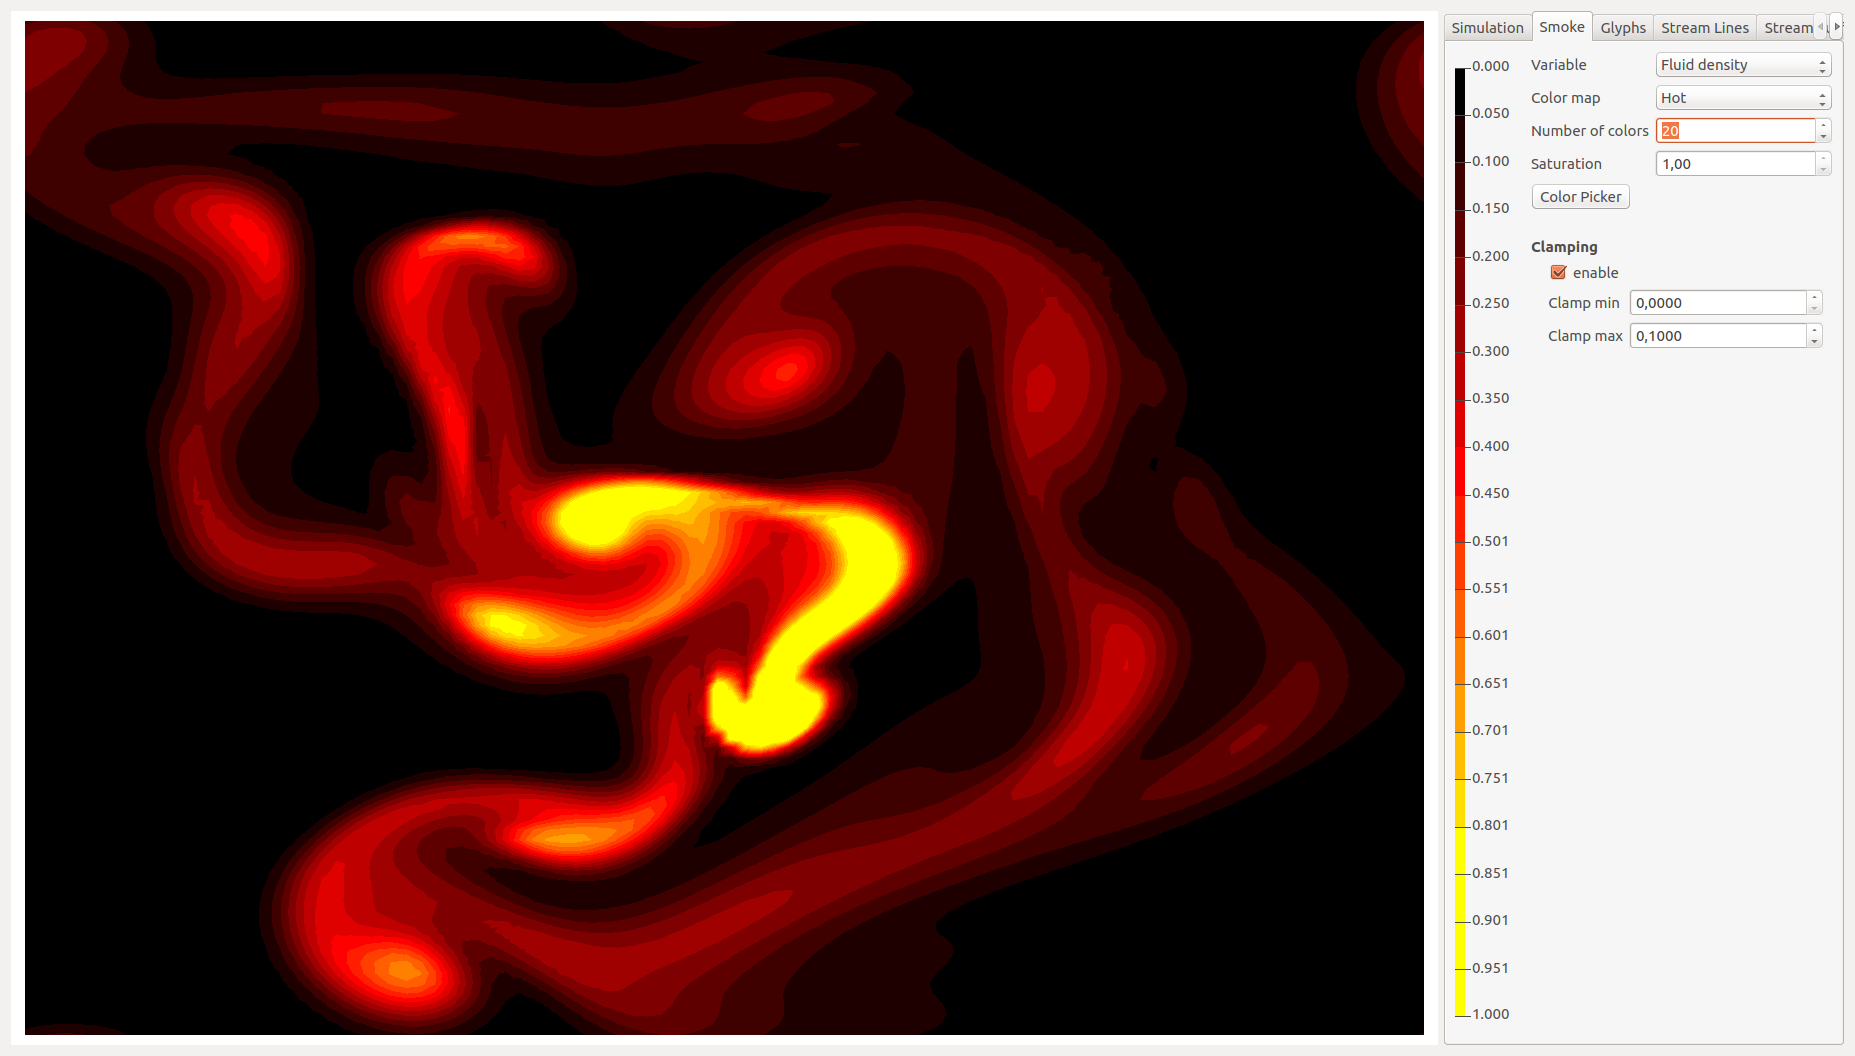
\includegraphics[width=\textwidth, trim={235px 30px 1230px 830px}, clip]{colormapping/img/heat20}
		\caption{Example of a visualization using a heat-map containing 20 colors.}
		\label{fig:colormapping:banding:20}
	\end{subfigure}
	\hspace{50px}
	\begin{subfigure}[t]{0.4\textwidth}
		\centering
		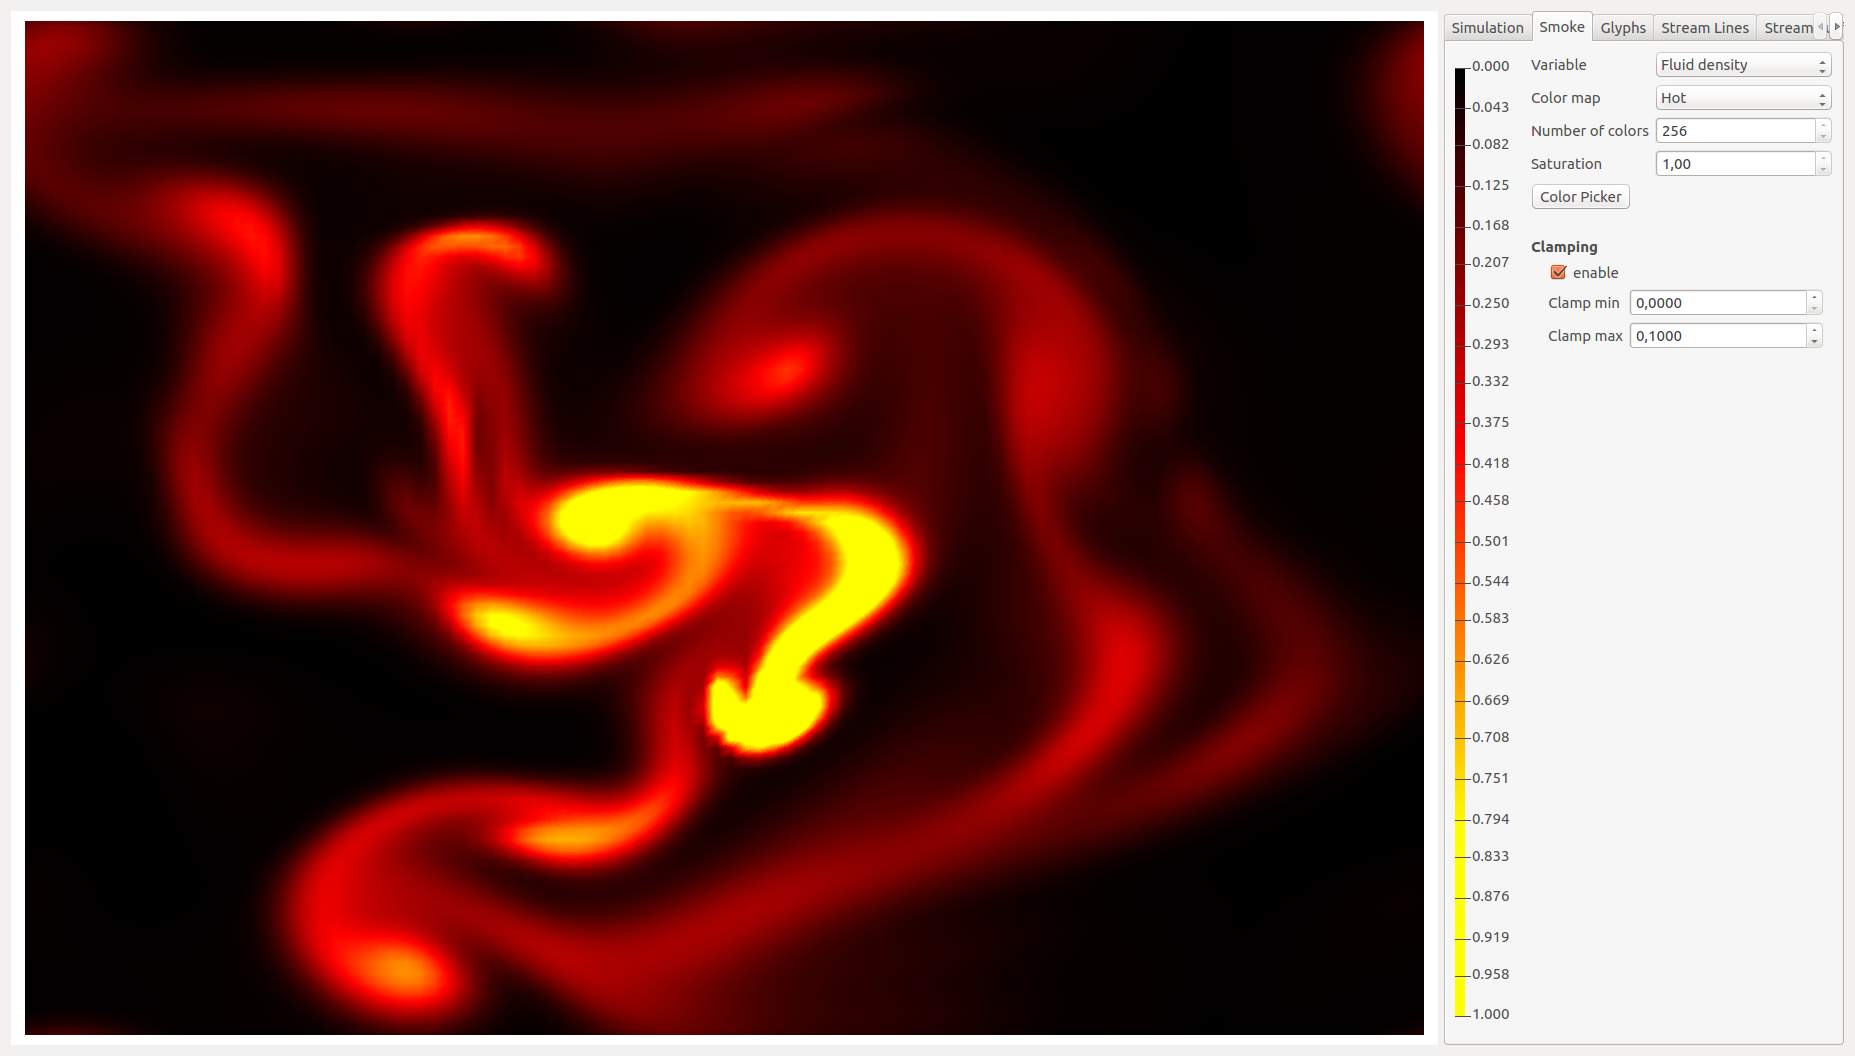
\includegraphics[width=\textwidth, trim={235px 30px 1230px 830px}, clip]{colormapping/img/heat256}
		\caption{Example of a visualization using a heat-map containing 256 colors.}
		\label{fig:colormapping:banding:256}
	\end{subfigure}	
	\caption{The influence of the number of colors in the colormap shown using the heat-map using 20 \subref{fig:colormapping:banding:20} and 256 \subref{fig:colormapping:banding:256} colors. Both images are taken from the same simulation state and zoomed in on the same location to show the effect more clearly.}
	\label{fig:colormaps:banding}
\end{figure}

\subsubsection{Saturation} % (fold)
\label{ssub:saturation}
Besides the number of colors it is also possible to change the saturation of (a subset of) the colormaps. Saturation influences the intensity of a color: colors with full saturation will appear pure, while colors with low saturation appear more washed out. Changing the saturation of a colormap can be of use when displaying multiple visualization techniques together. An example of the effect of changing saturation is given in \cref{fig:colormaps:saturation}. In \cref{fig:colormapping:saturation:disabled} the glyphs are almost non distinguishable from the scalar visualization but are made clearly visible in \cref{fig:colormapping:saturation:enabled} by lowering the saturation of the scalar visualization. In the application it is possible to change the saturation of most colormaps, however user should keep in mind that lowering the saturation can cause a less distinct ordering of the colors in the colormap.

\begin{figure}[tb]
	\centering
	\begin{subfigure}[t]{0.4\textwidth}
		\centering
		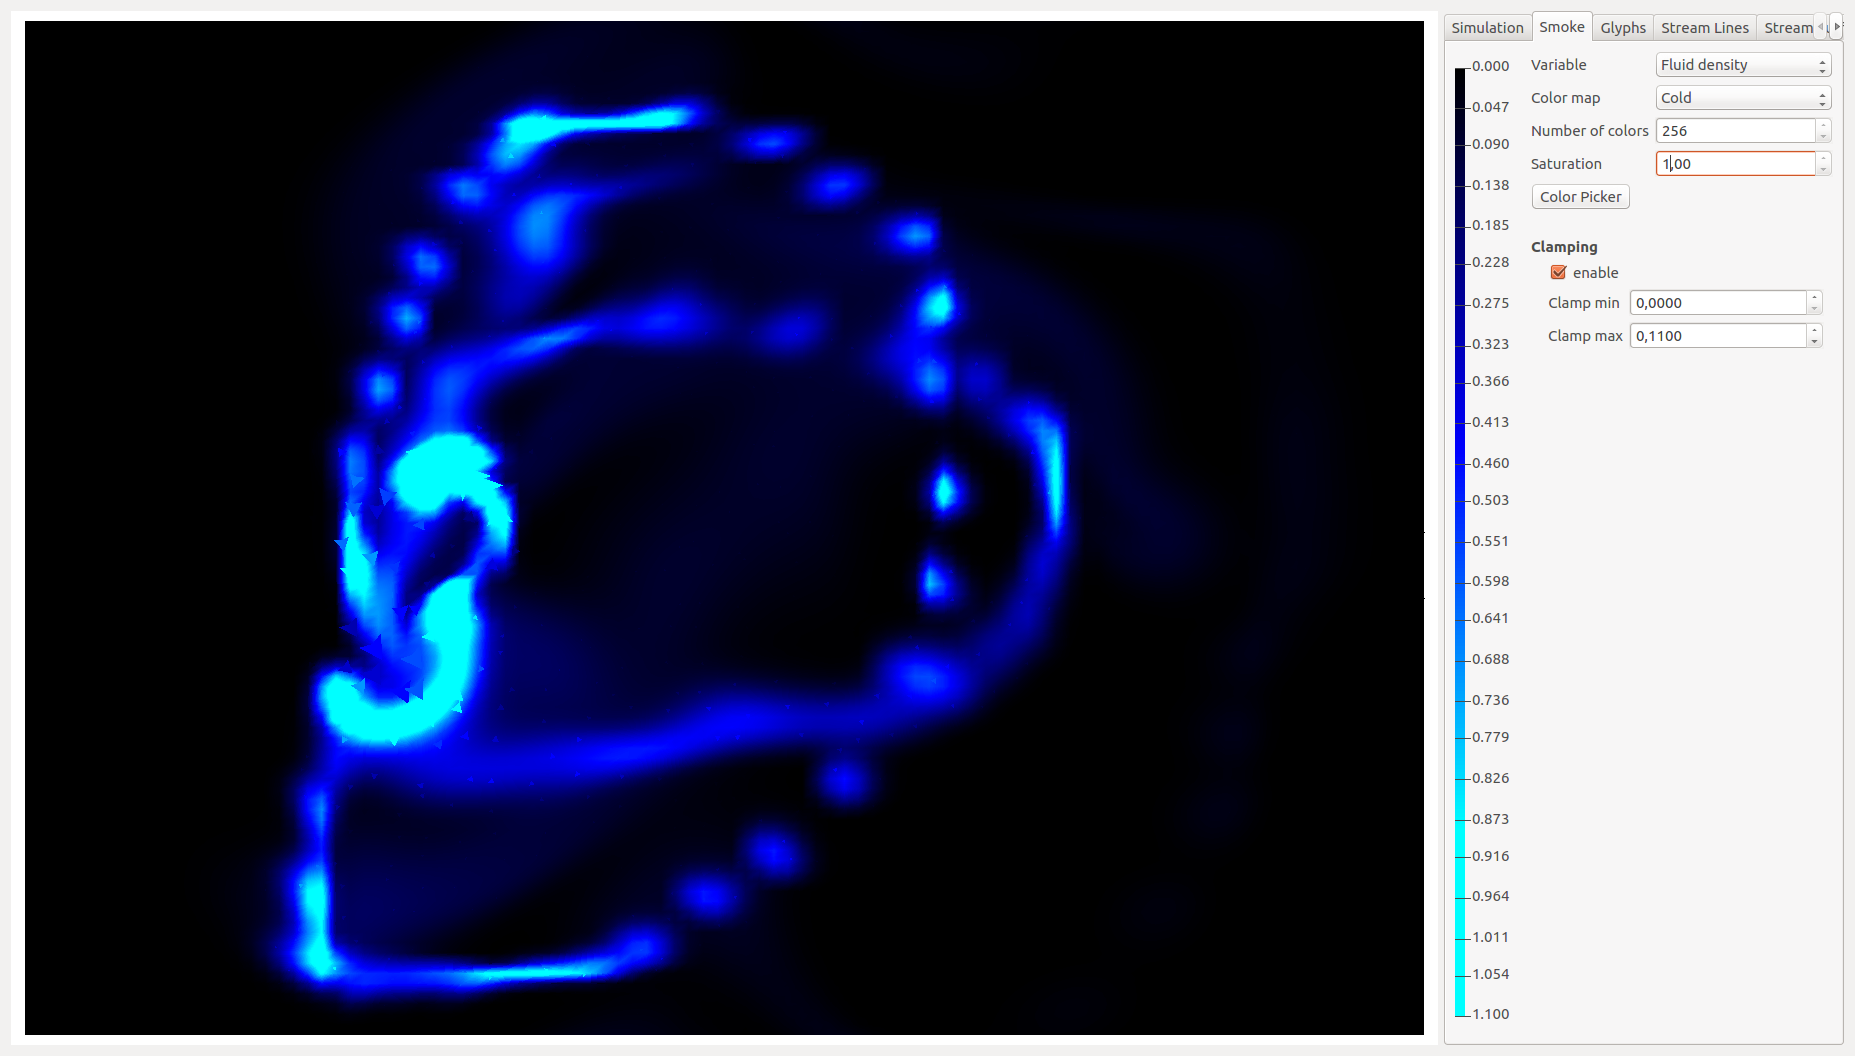
\includegraphics[width=\textwidth, trim={50px 200px 1023px 300px}, clip]{colormapping/img/nosaturation}
		\caption{Combination of scalar and vector visualization, both using the same fully saturated colormap.}
		\label{fig:colormapping:saturation:disabled}
	\end{subfigure}
	\hspace{50px}
	\begin{subfigure}[t]{0.4\textwidth}
		\centering
		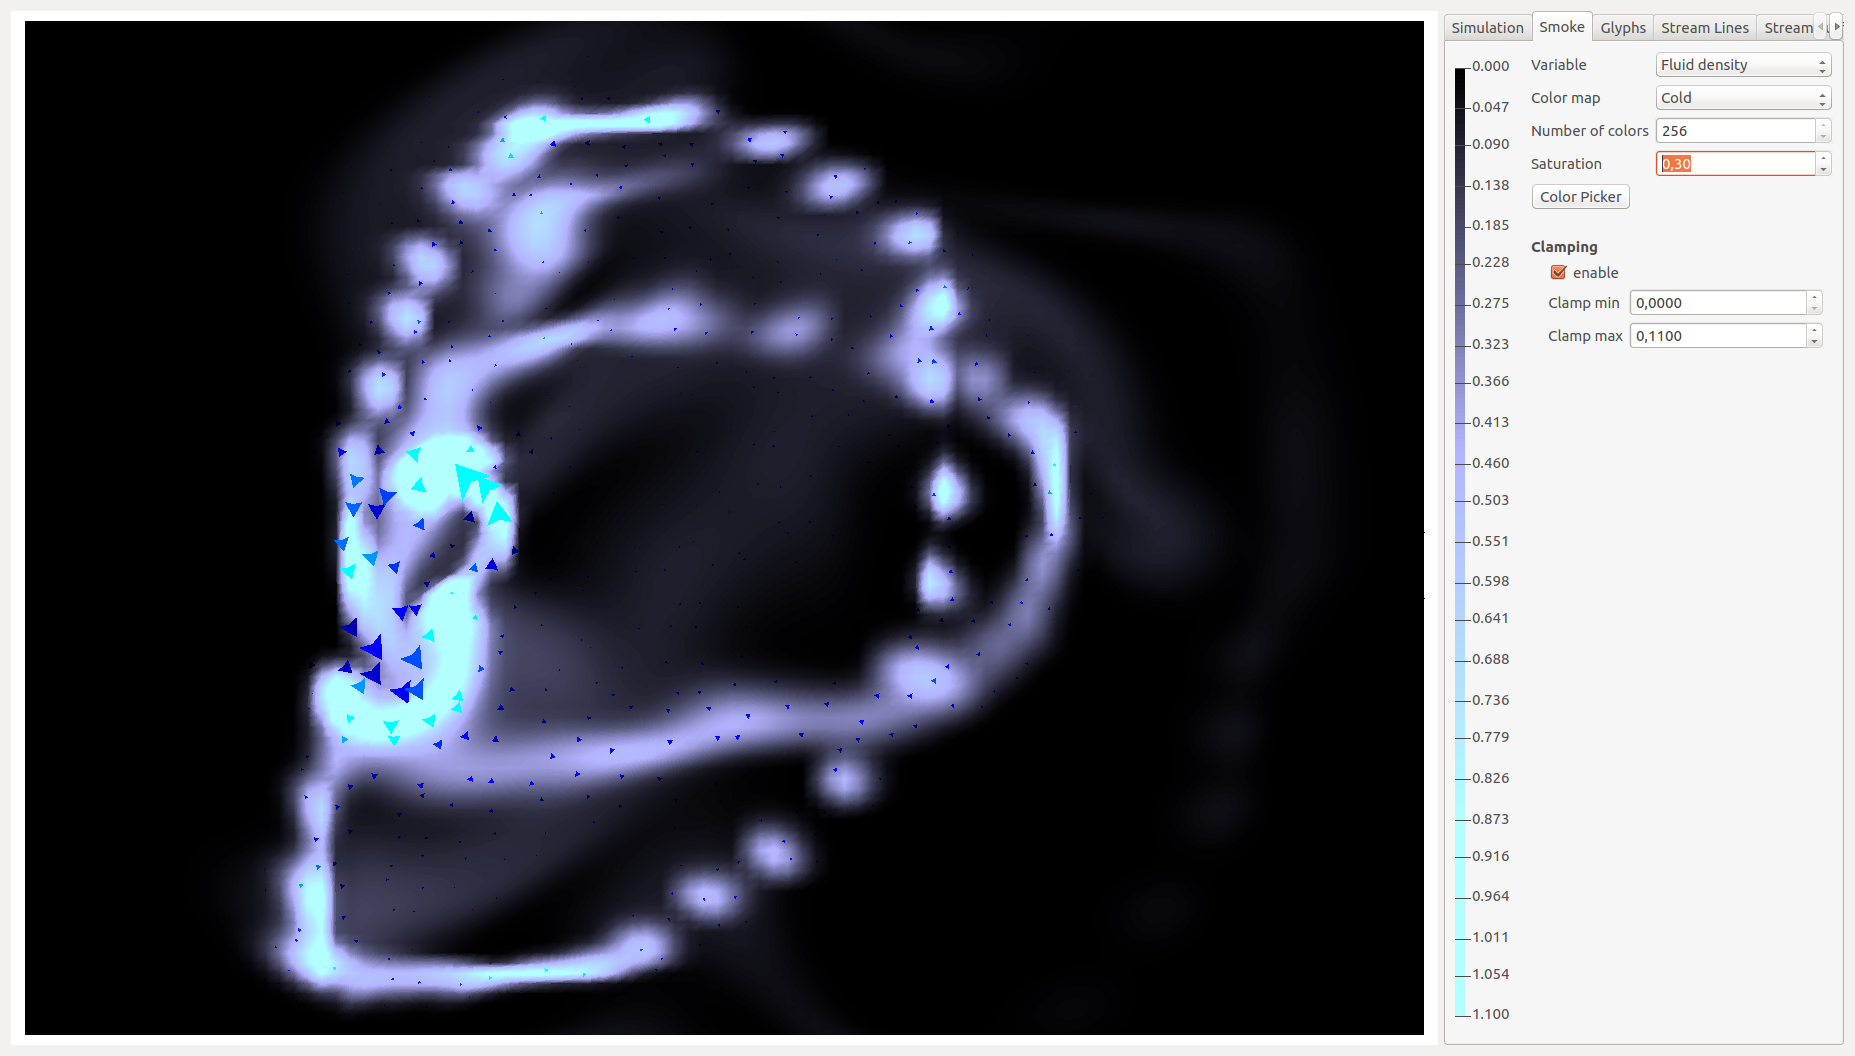
\includegraphics[width=\textwidth, trim={50px 200px 1023px 300px}, clip]{colormapping/img/saturation}
		\caption{Combination of scalar and vector visualization, the scalar visualization colormap has a saturation of $0.30$ and the vector visualization colormap is fully saturated.}
		\label{fig:colormapping:saturation:enabled}
	\end{subfigure}	
	\caption{Example of the influence of saturation when combining \smoke and vector visualization (see \cref{cha:glyphs}), using the same colormap for both visualization techniques. In \subref{fig:colormapping:saturation:disabled} the saturation of both colormaps is the same, while in \subref{fig:colormapping:saturation:enabled} the colormap of the scalar visualization has a lower saturation while the colormap of the vector visualization is still fully saturated. }
	\label{fig:colormaps:saturation}
\end{figure}

\subsection{Applying Colormaps}
\label{ss:colormaps:applying}
An important aspect of using colormaps is how they are applied to the scalar values. Given a colormap of $N$ colors with colors $c_1,c_2,\cdots,c_N$ and the (assumed) range of scalar values $[f_{min}, f_{max}]$, this range is mapped to the colormap by associating each scalar value between $[f_{min}, f_{max}]$ to a color in the colormap in increasing order (meaning lower $f$ values are mapped to colors with a lower index). The choice of $[f_{min}, f_{max}]$ is important when using a colormap. Imagine that we have picked $f_{min} = 0$ and $f_{ma} = 100$ but the actual range of the scalar values in the simulation is between $10$ and $20$. In this case the visualization would only display ten percent of the $N$ colors in the colormap. Ideally the entire range of the colormap is applied to the full range of scalar values in order not to `waste' parts of the colormap.

In our application $[f_{min}, f_{max}]$ can be set in two ways. The first method uses a fixed range of $f_{min} = 0$ and picks $f_{max}$ based on the scalar value visualized and the forces that are input by the user\footnote{Given an input force set to 10 we have (empirically) determined that the fluid density has $f_{max} = 10$, fluid velocity magnitude has $f_{max} = 0.1$, and the force field magnitude has $f_{max} = 0.1$.}. These $[f_{min}, f_{max}]$ are kept constant during the entire simulation. This has as advantage that it is easier to observe the change in scalar values over time but has the disadvantage that after some time-steps in which there are no new forces added to the simulation, the range of the scalar values only uses a small subset of the colormap, making the differences between scalar values not prominent.

The second method uses a dynamic range $[f_{min}, f_{max}]$. This is done by determining the min and max of the visualized scalar data for every time-step in the simulation and $[f_{min}, f_{max}]$ are changed accordingly. This has as big advantage that every time-step the full range of the colormap is used. The disadvantage is that it is harder to determine the change in scalar values over time.

\subsubsection{Clamping} % (fold)
\label{ssub:clamping}
In the section above we assumed that the scalar values were uniformly distributed in their range. However, some simulations might result in non-uniformly distributed scalar values, e.g. most scalar values fall within a range much smaller than $[f_{min}, f_{max}]$. In these cases it might be desirable to use show more detail in the range that contains the most scalar values. To facilitate this the user can adapt $[f_{min}, f_{max}]$ to a range $[f^{clamp}_{min}, f^{clamp}_{max}]$ such that $f_{min} \leq f^{clamp}_{min}$ and $f_{max} \geq f^{clamp}_{max}$\footnote{At all times it is ensures that lower clamping bound is less than the upper clamping bound.}. Scalar values outside the range $[f^{clamp}_{min}, f^{clamp}_{max}]$ are clamped to the edge of the colormap. This has as disadvantage that it is not possible to distinguish between scalar values outside of the clamping range, but offers better resolution inside this range. An example of clamping is given in \cref{fig:colormapping:clamped}, here the clamped variant shows much more detail but shows the same color for all scalar values between $0.1$ and $10$.

\begin{figure}[tb]
	\centering
	\begin{subfigure}[t]{0.4\textwidth}
		\centering
		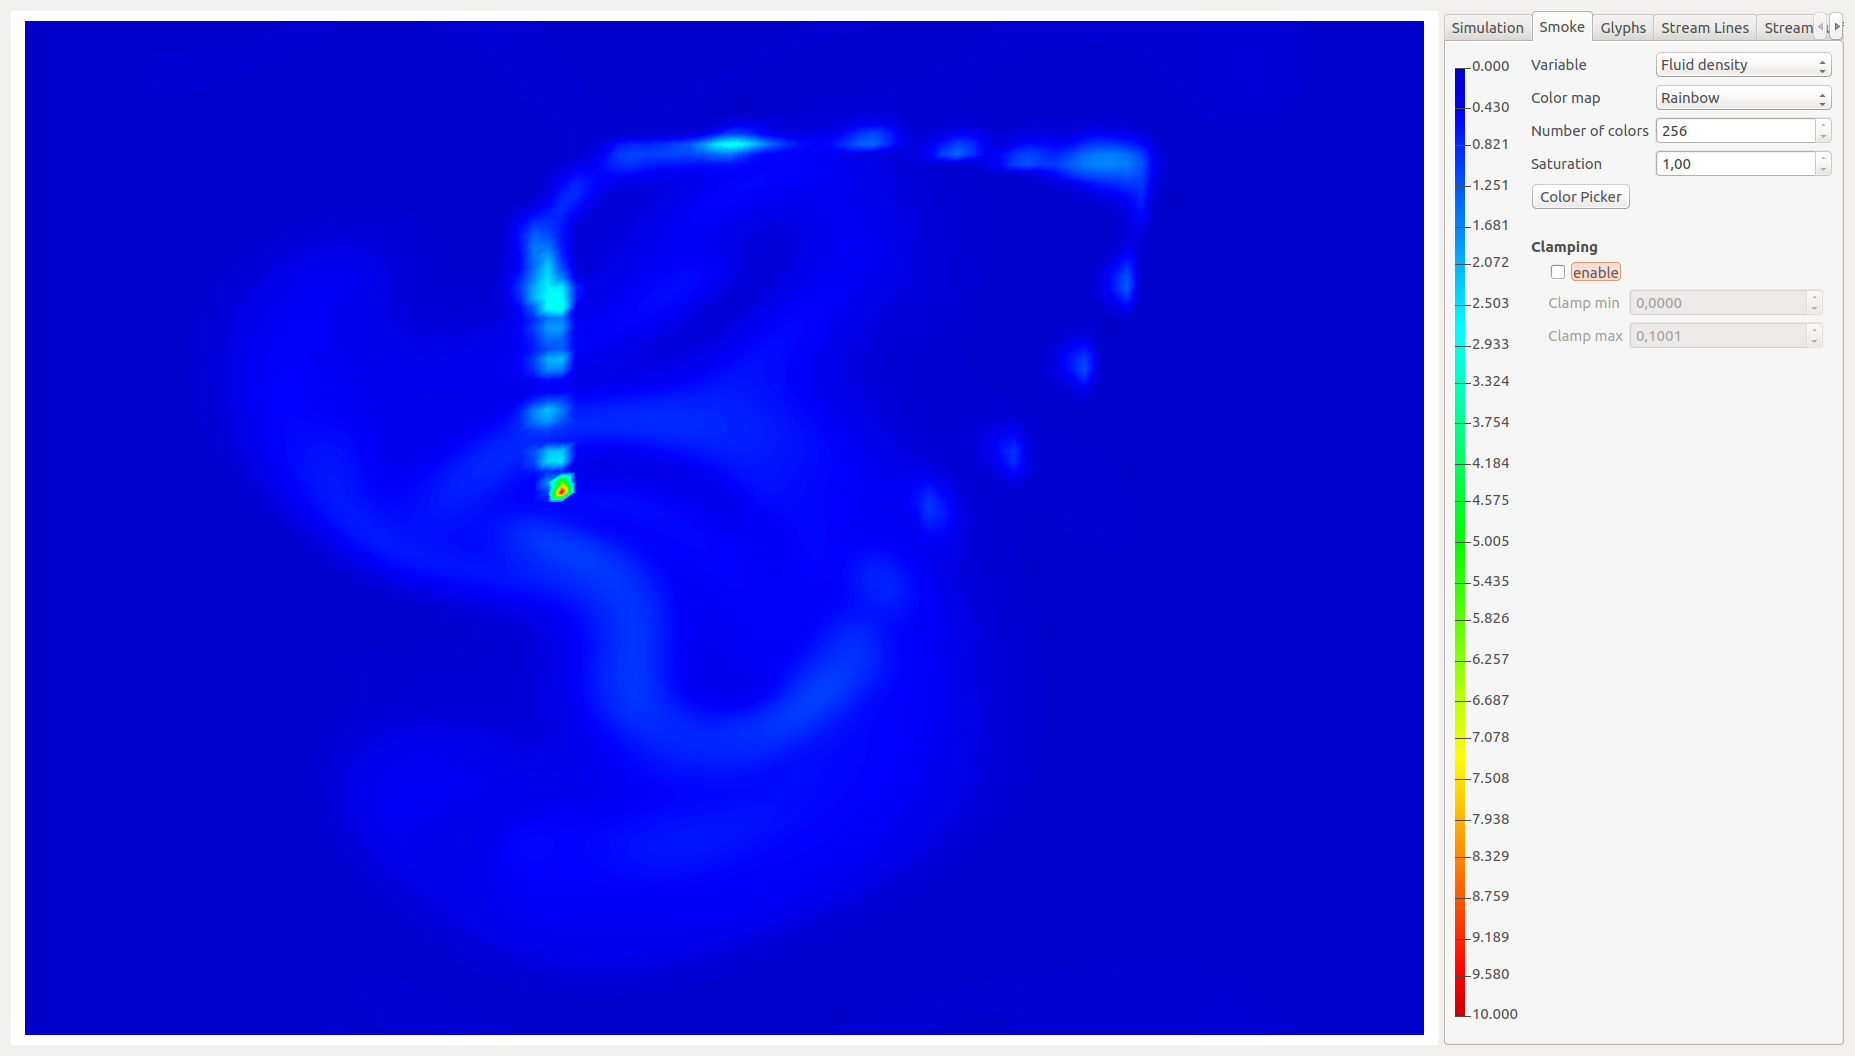
\includegraphics[width=\textwidth, trim={35px 30px 430px 30px}, clip]{colormapping/img/notclamped}
		\addrainbow{0.0}{10}
		\caption{Visualization of the scalar values without clamping using the rainbow colormap.}
		\label{fig:colormapping:clamped:disabled}
	\end{subfigure}
	\hspace{50px}
	\begin{subfigure}[t]{0.4\textwidth}
		\centering
		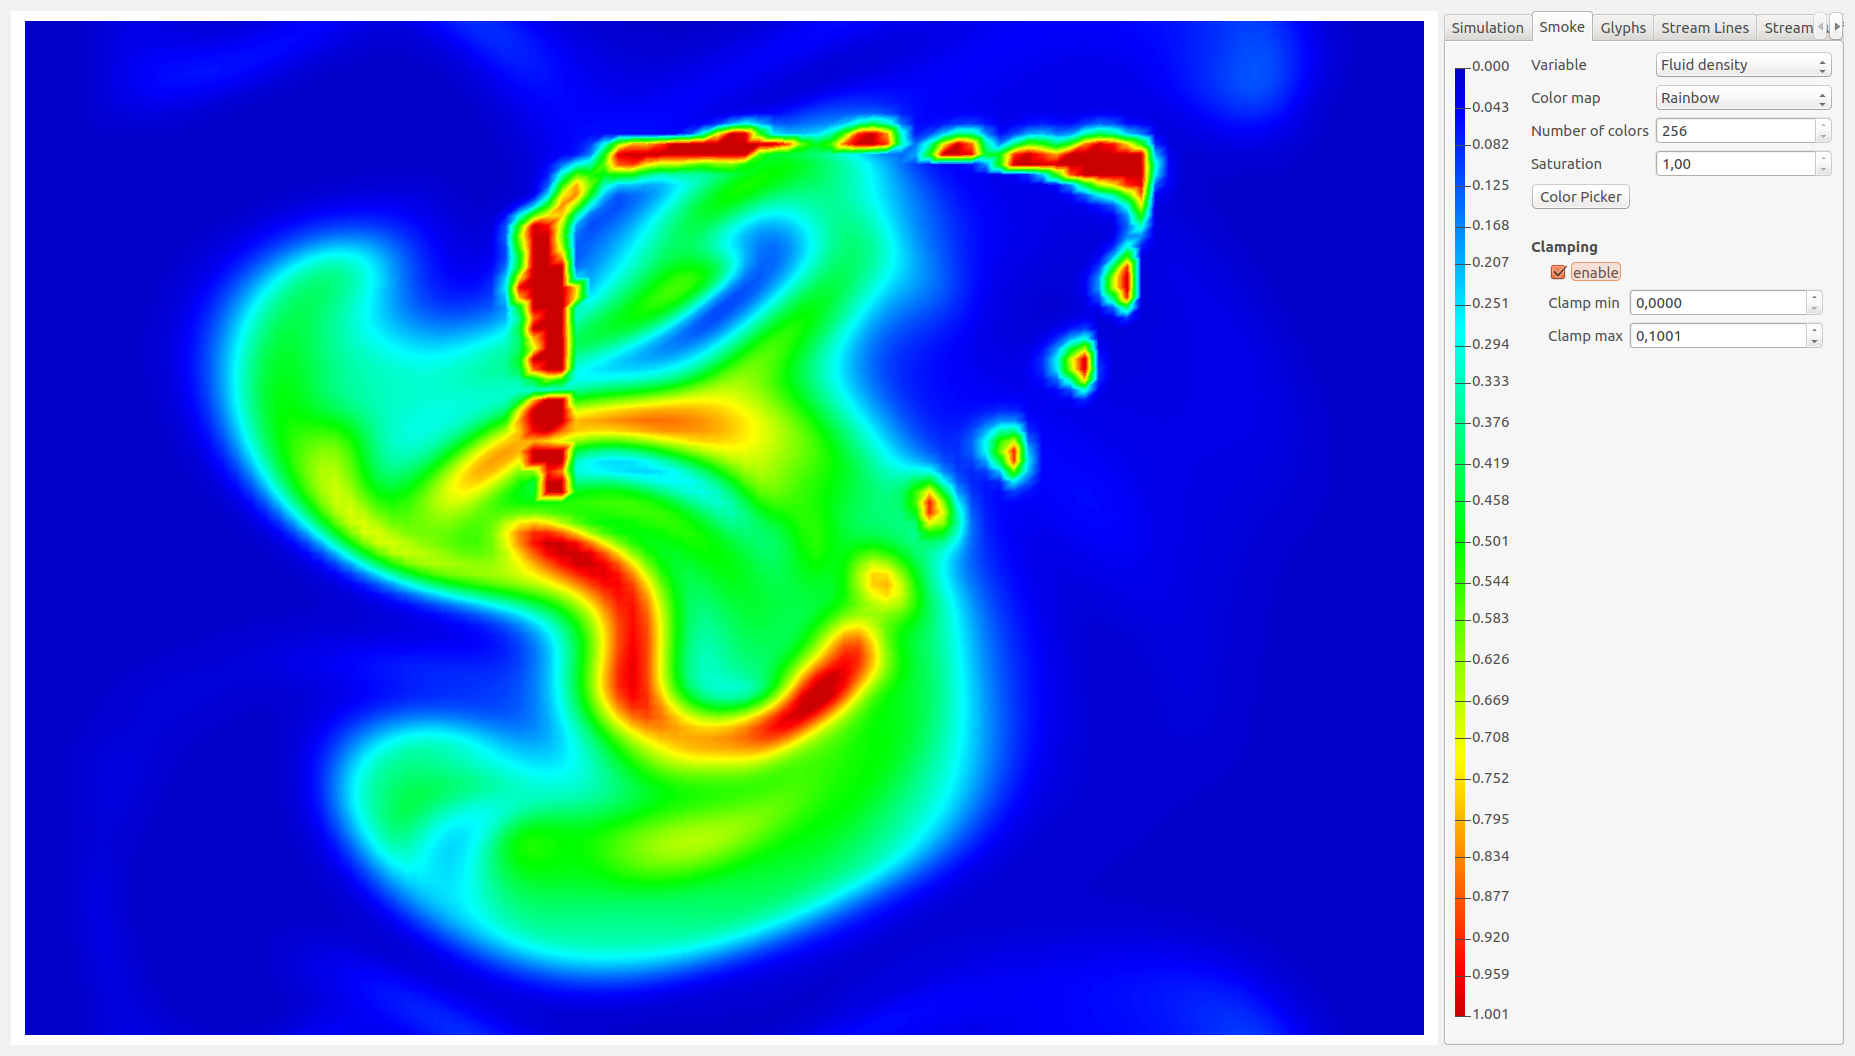
\includegraphics[width=\textwidth, trim={35px 30px 430px 30px}, clip]{colormapping/img/clamped_01}
		\addrainbow{0.0}{0.1}
		\caption{Visualization of the scalar values with clamping using the rainbow colormap with $f^{clamp} = 0.1 f_{max}$.}
		\label{fig:colormapping:clamped:enabled}
	\end{subfigure}	
	\caption{Example of a visualization with and without clamping of $f_{max}$. The clamped version (figure \subref{fig:colormapping:clamped:enabled}) shows more detail but does not discriminate scalar values above $0.1$.}
	\label{fig:colormapping:clamped}
\end{figure}